\documentclass[../jarvis.tex]{subfiles}
\graphicspath{{\subfix{../images/}}}
\begin{document}
Outside of quadratic polynomials, there are also cubics, quartics, quintics, sextics..., that most students assume are extinct. However, they can be found in a select number of natural hideouts! In this handout, we look at the structures associated with polynomials, as well as the techniques to deal with them. 

\begin{figure}[H]
    \centering
    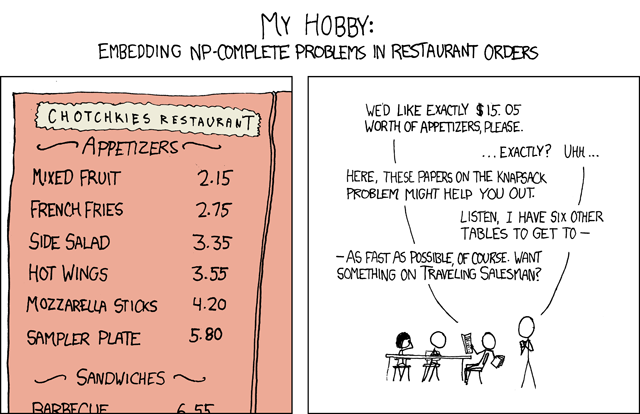
\includegraphics[scale=7]{xkcd_np_complete.png}
    \caption{Comic from https://xkcd.com/287/}
\end{figure}
\section{Quadratics \ez}
In this section, we will revisit the common quadratic polynomials.
The techniques for quadratics aren't many. The usual few are the discriminant and completing the square, none of which are totally unexpected or inspiring. However, they are still useful-ish in extracting information from a given problem.

\subsection{Algebraic Properties of Quadratics \ez}
We begin by stating some algebraic properties of the quadratic curve. In what follows, let $$P(x)=ax^2+bx+c=a\left(x+\frac{b}{2a}\right)^2+\left(c-\frac{b^2}{4a}\right).$$
\begin{proposition}[Quadratic Formula]
    The two (not necessarily distinct) roots of $P(x)$ is given by the \textit{quadratic formula}
    $$x=\frac{-b\pm\sqrt{b^2-4ac}}{2a}.$$
\end{proposition}
\begin{proof}
    Consider the completed square form, then 
    \begin{align*}
        P(x)=0 &\iff a\left(x+\frac{b}{2a}\right)^2+\left(c-\frac{b^2}{4a}\right)=0 \\
        &\iff a\left(x+\frac{b}{2a}\right)^2=\frac{b^2}{4a}-c \\
        &\iff \left(x+\frac{b}{2a}\right)^2=\frac{b^2-4ac}{4a^2} \\
        &\iff x+\frac{b}{2a}=\frac{\pm\sqrt{b^2-4ac}}{2a} \\
        &\iff x=\frac{-b\pm\sqrt{b^2-4ac}}{2a}
    \end{align*}
\end{proof}
\begin{proposition}[Discriminant]
    The discriminant is given by $\Delta=b^2-4ac$.
\end{proposition}
Observe that $\Delta$ lies under the square root in the numerator of the quadratic formula. Hence, if $\Delta>0$, there are two distinct roots. If $\Delta=0$, the root is simply $x=-\frac{b}{2a}$.

The special case is if $\Delta<0$, then we have two complex roots. This also says that complex roots come in \textit{conjugate pairs}, that is if
$$x_1=\frac{-b}{2a}\pm\frac{\sqrt{|b^2-4ac|}}{2a}i$$
is a root, then so is
$$x_2=\frac{-b}{2a}\mp\frac{\sqrt{|b^2-4ac|}}{2a}i.$$

\subsection{Geometric Properties of Quadratics}
The quadratic is also miraculous in that it is symmetric about it's \textbf{vertex}.

The graphical behaviour of a quadratic depends largely on its \textbf{leading coefficient}, that is the coefficient of the highest degree term. For $P(x)$, the leading coefficient is $a$.

Indeed, for large values of $x$, $P(x)$ is \textbf{dominated} by the term $ax^2$. If $a>0$, then $P(x)$ tends to positive infinity, that is, the graph opens \textbf{upwards}. On the other hand, if $a<0$, then $P(x)$ tends to negative infinity, that is, the graph opens \textbf{downwards}.

\begin{figure}
    \centering
    \begin{minipage}{.5\textwidth}
      \centering
      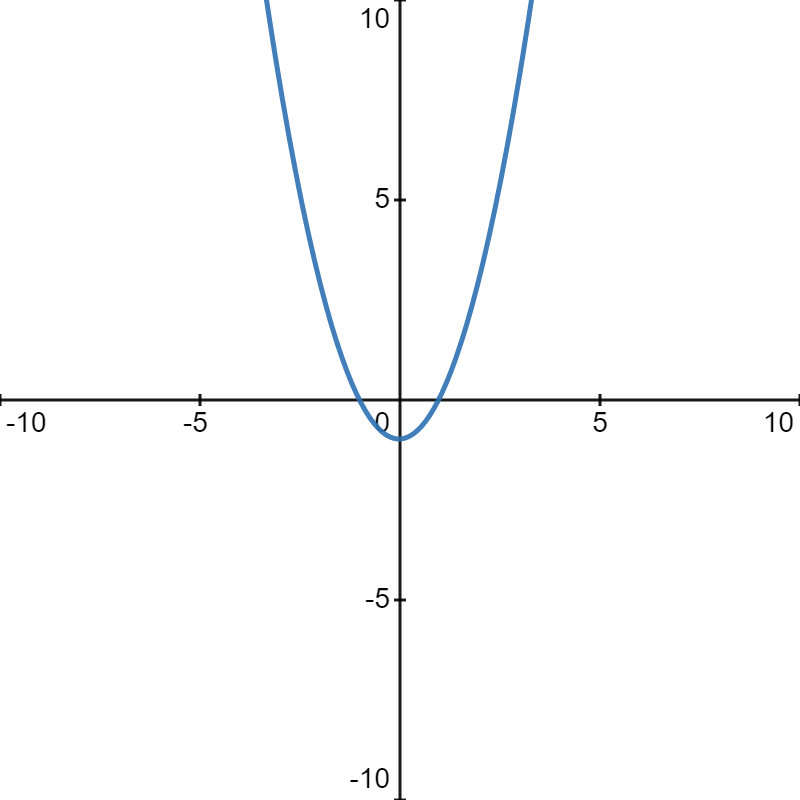
\includegraphics[width=.7\linewidth]{quadratic_up.png}
      \caption{For $a>0$.}
    \end{minipage}%
    \begin{minipage}{.5\textwidth}
      \centering
      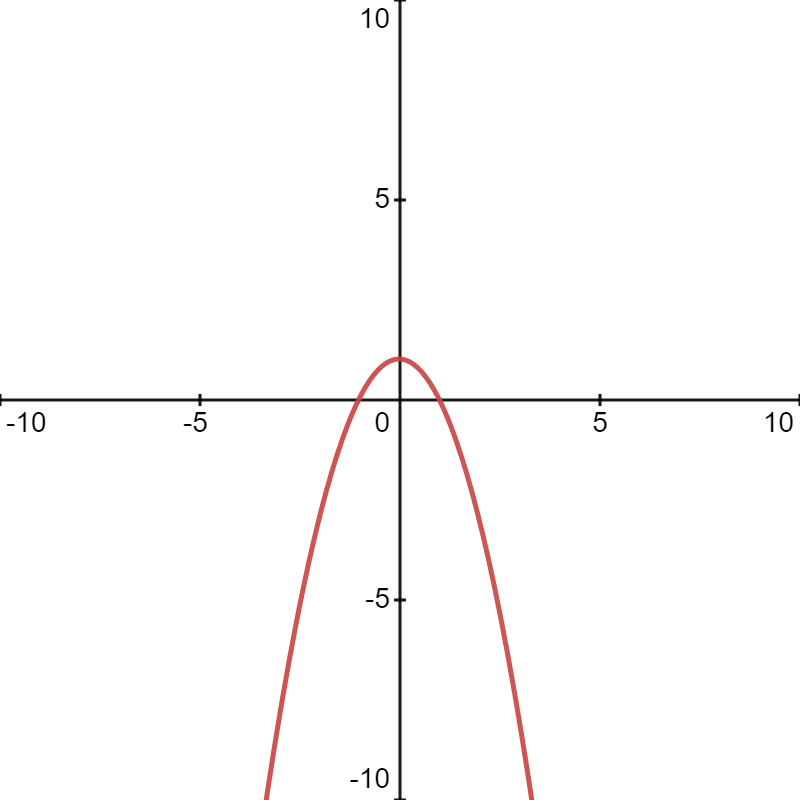
\includegraphics[width=.7\linewidth]{quadratic_down.png}
      \caption{For $a<0$.}
    \end{minipage}
\end{figure}

From the graph, one can also observe that the quadratic curve is \textbf{symmetric}. Crucially, it is symmetric about it's vertex, that is, the maximum or minimum point of the quadratic, depending on whether $a$ is positive or negative. We first discover the coordinates of the vertex.
\begin{proposition}[Coordinates of the Vertex]
    The vertex occurs at $x=\frac{b}{2a}$.
\end{proposition}
\begin{proof}
    Consider again the completed square form. Then,
   \begin{align*}
        P(x)&=a\left(x-\frac{b}{2a}\right)^2+\left(c-\frac{b^2}{4a}\right) \\
        &\geq c-\frac{b^2}{4a},
   \end{align*}
   because $\left(x-\frac{b}{2a}\right)^2\geq 0$. This leads us to the most important inequality for any polynomial: \textbf{the trivial inequality}.
   \begin{proposition}[The Trivial Inequality]
       For any real $x$, $x^2\geq 0$.
   \end{proposition}
   This is easily seen by considering the graph $y=x^2$, and noting that it is tangent to the line $y=0$. 
   
   Moreover, we make the crucial observation that \textbf{\textit{any} quadratic curve is simply a scaled and translated copy of the curve $y=x^2$}.

   This means that the minimum value of the quadratic is $y=c-\frac{b^2}{4a}$, and this value is achieved when $$\left(x-\frac{b}{2a}\right)^2=0 \implies x=\frac{b}{2a}.$$

   In other words, the coordinates of the vertex is $$\left(-\frac{b}{2a},c-\frac{b^2}{4a}\right).$$
\end{proof}
Moreover, the vertex is the point of symmetry. To illustrate, let $A$ and $C$ be two points that lie on the same horizontal line such that $A$ and $C$ are on different \textit{arms} of the curve. Then, the distance from $A$ to the line of symmetry and the distance from $C$ to the same line is equal.

In other words, $|AB|=|BC|$.
\begin{figure}[H]
    \centering
    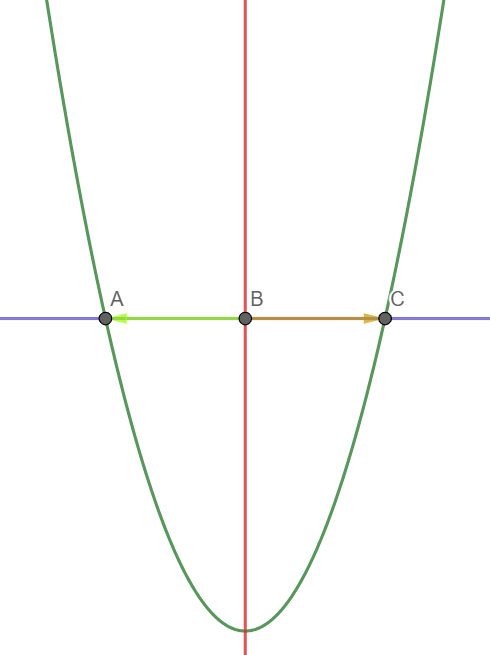
\includegraphics[scale=0.5]{quadratic_symmetry.PNG}
    \caption{Equidistance from the line of symmetry.}
\end{figure}

This property is independent of the constant term since the constant term only affects the \textit{upwards and downwards} shift of our quadratic graph. Hence, we shall ignore it and assume for convenience that the constant term is $0$. This means that for simplicity, we can simply assume that any quadratic curve has a vertex that lies exactly on the $x$-axis. And again, this is a legal assumption because the constant term does not affect our line of symmetry!

We now make use of our crucial observation that any quadratic is simply a scaled and translated version of $y=x^2$. Henceforth, let $Q(x)=\left(x-\frac{b}{2a}\right)^2$ (this is $P(x)$ without a constant term).

We note that the curve $y=x^2$ has a vertical line of symmetry at $x=0$. Thus, we obtain $Q(x)$ by \textbf{translating} the graph of $y=x^2$ by $\frac{b}{2a}$ units to the \textit{right} of the cartesian plane.

In formal terms, we say that $Q(x)$ is obtained by \textbf{translating} the graph of $y=x^2$ by $\frac{b}{2a}$ units \textbf{in the direction of the positive $x$-axis}. 

It is then a simple consequence of this symmetry that the $x$-coordinate of the vertex is the average of the roots of the quadratic. Indeed, let $r_1$ and $r_2$ be the roots, then
\begin{align*}
    r_1+r_2&=\left(-\frac{b}{2a}+\frac{\sqrt{\Delta}}{2a}\right)+\left(-\frac{b}{2a}-\frac{\sqrt{\Delta}}{2a}\right)=-\frac{b}{a}.
\end{align*}
\subsection{Roots of a Quadratic \ez}
With the basics and fundamentals out of the way, let us see how the algebraic and geometric properties play together nicely.
\begin{example}[2010-2011 Mandelbrot]
    Let $P(x)=x^3+ax^2+bx+c$ be a polynomial with three distinct roots. The polynomial P(Q(x)), where $Q(x)=x^2+x+2001$, has no real roots. Prove that $P(2001)>\frac{1}{64}$.
\end{example}
This is a strange idea: given the number of roots of a polynomial, what can we deduce about it's value?

\begin{proof}
    For starters, let $p,q,r$ be the three distinct roots of $P$, then $P(x)=(x-p)(x-q)(x-r)$ and let $z$ be a complex root of $P(Q(x))$ so that $P(Q(z))=0$. 

Hence, $Q(z)=\text{$p$ or $q$ or $r$}$. Without loss of generality, $$Q(z)=p \implies z^2+z+(2001-p)=0.$$

However, there are no real values of $z$ that satisfy this condition! This next step would be glaring: by considering the discriminant,
$$\Delta=1-4(2001-p) < 0 \implies p < \frac{8003}{4}.$$

Since we initially assumed without loss of generality that $Q(z)=p$, this conclusion should also hold for $q, r$, that is $p,q,r < \frac{8003}{4}$.

Finally, \begin{align*}
    P(2001)=(2001-p)(2001-q)(2001-r) &> \frac{1}{4}\cdot\frac{1}{4}\cdot\frac{1}{4} \\
    &=\frac{1}{64}
\end{align*}
\end{proof}
Next, we consider a quadratic with coefficients that form an arithmetic progression. As it turns out, if the quadratic has a unique root, then we can uniquely determine this root!
\begin{example}[2013 AMC 10B P19]
    Let $c,b,a$ be real numbers form an arithmetic progression with $a\geq b\geq c\geq 0$. The quadratic $ax^2+bx+c=0$ has exactly one root. Find this root.
\end{example}
First step! Our only root is $x=\frac{-b}{2a}$.

\begin{proof}
    Since $c,b,a$ have common differences with $b$ being the median element, we may write $c=2b-a$ so that 
$$b^2-4ac=b^2-4a(2b-a)=b^2-8ab+4a^2=0 \implies b=4a\pm2a\sqrt{3}.$$
Yet, we are given that $a\geq b$, so surely $b=4a-2a\sqrt{3}$, giving $x=-\frac{b}{2a}=\boxed{-2+\sqrt{3}}.$
\end{proof}

\section{Vieta's Theorem and Higher Ordered Polynomials \med}
Contrary to popular belief, there are higher degree polynomials in the wild. We first consider some identities associated with the coefficients of a general polynomial.

Consider a general polynomial $$P(x)=a_nx^n+a_{n-1}x^{n-1}+\cdots+a_1x+a_0$$ with real coefficients $\{a_n\}$. Then, the
\begin{enumerate}
    \item constant term is $P(0)$,
    \item sum of coefficients is $P(1)$,
    \item sum of \textit{odd-power} coefficients is $\frac{P(1)-P(-1)}{2}$,
    \item sum of \textit{even-power} coefficients is $\frac{P(1)+P(-1)}{2}$.
\end{enumerate}

The reader is strongly encouraged to derive the four properties above!

For the other coefficients, there are other higher-powered techniques (pun fully intended) to deal with them, but we will not introduce them here (for the interested, see the roots of unity filter).

We are guessing the student is familiar with the so-called "sum and product of roots" for a quadratic, and here, we introduce a generalisation - we have similar relations for higher-degree polynomials! This is given by Vieta's Theorem.

\begin{proposition}[Vieta's Theorem]
    A general polynomial $P(x)=a_nx^n+a_{n-1}x^{n-1}+\cdots+a_1x+a_0$ with real coefficients $\{a_n\}$ and real and complex roots $r_1, r_2, \cdots r_n$ has the following relations:
    \begin{align*}
        r_1+r_2+\cdots+r_n&=-\frac{a_{n-1}}{a_n}\\
        (r_1r_2+r_1r_3+\cdots+r_1r_n)+(r_2r_3+r_2r_4+\cdots+r_2r_n)+\cdots+r_{n-1}r_n&=\frac{a_{n-2}}{a_n} \\
        r_1r_2\cdots r_n=(-1)^n\frac{a_0}{a_n}
    \end{align*}
    In general, the \textit{sum of roots taken k at a time} is given by $(-1)^k\frac{a_{n-k}}{a_n}.$ Each of these sums are also known as \textit{elementary symmetric polynomials}.
\end{proposition}

Let us show some examples of Vieta's theorem in action. 
\begin{example}[2001 All-Russian Olympiad]
    The equation $(x-\sqrt[3]{13})(x-\sqrt[3]{53})(x-\sqrt[3]{103})=\frac{1}{3}$ has three distinct roots $r,s,t$. Find the value of $r^3+s^3+t^3$.
\end{example}

First of all... yikes! Cube roots and cubes. However, it seems that the three cube roots look arbitrary: while the answer depends on their values, we can find an expression for $r^3+s^3+t^3$ in terms of these cube roots without caring about their values just yet. 
\begin{proof}
    We make the substitution $a=\sqrt[3]{13}$, $b=\sqrt[3]{53}$, $c=\sqrt[3]{103}$, so that our equation is transformed into $$(x-a)(x-b)(x-c)-\frac{1}{3}=0$$. By Vieta's theorem, 
\begin{align*}
    r+s+t&=a+b+c \\
    rs+st+rt&=ab+bc+ca \\
    rst&=abc-\frac{1}{3}.
\end{align*}
Now, how do we use this to our advantage to find $r^3+s^3+t^3$? For starters, we may expand
$$(r+s+t)^3=r^3+s^3+t^3+3r^2s+3r^2t+3rs^2+3rt^2+3s^2t+3st^2+6rst.$$
We're close to finding something substantial - if we can simplify the sum of the terms in the form $m^2n$. A natural way to do this is to expand
$$(r+s+t)(rs+st+rt)=r^2s+r^2t+rs^2+rt^2+s^2t+st^2+3rst.$$

Aha! Now our expression simplifies nicely:
$$(r+s+t)^3=r^3+s^3+t^3+3(r+s+t)(rs+st+rt)-3rst,$$
whence upon arranging, we have
\begin{align*}
    r^3+s^3+t^3
    &=(\alpha+\beta+\gamma)^3-3(\alpha+\beta+\gamma)(\alpha\beta+\beta\gamma+\gamma\alpha)+3(\alpha+\beta+\gamma+\frac{1}{3})\\
    &=(\alpha+\beta+\gamma)^3-3(\alpha+\beta+\gamma)(\alpha\beta+\beta\gamma+\gamma\alpha)+3(\alpha+\beta+\gamma)+1 \\
    &=\alpha^3+\beta^3+\gamma^3+1 \\
    &=\boxed{170}
\end{align*}
\end{proof}

\begin{example}[2019 AIME I P10]
For complex numbers $z_1, z_2,\cdots z_{673}$, the polynomial
$$(x-z_1)^3(x-z_2)^3\cdots(x-z_673)^3$$
can be expressed as $x^{2019}+20x^{2018}+19x^{2017}+g(x)$ where $g(x)$ is a polynomial with complex polynomials and of degree \textit{at most} $2016$. Find the value of 
$$\sum_{1\leq j\leq k\leq 673}z_jz_k.$$
\end{example}
The sum requested of us is an elementary symmetric polynomial, so we would expect to use Vieta's theorem in some way.

Let $S, P$ denote the sum of roots one and twice at a time respectively and let $Q(x)$ denote the given polynomial. Note that the required sum is $P$. Since it's weird that the given polynomial is cubed throughout, we shall consider
$$p(x)=(x-z_1)(x-z_2)\cdots(x-z_{673})=x^{673}-Sx^{672}+Px^{671}+\cdots$$

Thus, $Q(x)=[p(x)]^3$. To find $S$ and $P$, we shall expand this to find the coefficients of $x^{2018}$ and $x^{2017}$. To do this quickly, we consider how terms in 3 products can be multiplied together to give the relevant terms.

To wit, 
\begin{enumerate}
    \item $x^{2019}$ can only be formed by multiplying all three $x^{673}$, and there is only 1 way to do this.
    \item $x^{2018}$ can be formed by multiplying two $x^{673}$ and one $Sx^{672}$, and there are $\binom{3}{1}=3$ ways to do this.
    \item $x^{2017}$ can be formed by multiplying two $x^{673}$ and one $Px^{671}$, and there are $\binom{3}{1}=3$ ways to do this. It can also be formed by multiplying one $x^{673}$ and two $Sx^{672}$, giving $3$ ways as well.
\end{enumerate}
\begin{proof}
    We now have,
\begin{align*}
    Q(x)=[p(x)]^3&=(x^{673}-Sx^{672}+Px^{671}+\cdots)(x^{673}-Sx^{672}+Px^{671}+\cdots)(x^{673}-Sx^{672}+Px^{671}+\cdots) \\
    &= x^{2019}-3Sx^{2018}+3(P+S^2)x^{2017}+g(x),
\end{align*}
and thus
$$\begin{cases} -3S=20 \\ 3(P+S^2)=19 \end{cases}\Rightarrow \begin{cases} S=-\frac{20}{3} \\ P=-\frac{343}{9}\end{cases}.$$

Hence, $\boxed{P=-\frac{343}{9}}$.
\end{proof}

At this point, it's only complete if we also derive some common algebraic identities and factorisations. 
\begin{proposition}[Classic]
    In what follows, assume the summation run over $x_1,x_2,\cdots,x_n$.
    \begin{enumerate}
        \item For the bivariate $x^2+y^2=(x+y)^2-2xy$, we also have the three-variable relation $$x^2+y^2+z^2=(x+y+z)^2-2(xy+yz+zx).$$
        In general, $$\left(\sum x_i\right)^2=\sum x_i^2-2\left(\sum_{1\leq i\leq q\leq n}x_ix_j\right).$$

        \item $x^3+y^3+z^3-3xyz=\frac{1}{2}(x+y+z)[(x-y)^2+(y-z)^2+(z-x)^2]$.
        This also implies $$x^3+y^3+z^3 \geq 3xyz,$$ because
        $(x-y)^2+(y-z)^2+(z-x)^2\geq 0$.
        \item Sophie-Germain Identity: $a^4+4b^4=(a^2+2b^2+2ab)(a^2+2b^2-2ab)$.
        \item Lagrange's Identity: $(a^2+b^2)(c^2+d^2)=(ac-bd)^2+(ad+bc)^2=(ac+bd)^2+(ad-bc)^2$
        \item $(a+b)^3-(a^3+b^3)=3ab(a+b)$.
        \item $(a+b)^5-(a^5+b^5)=5ab(a+b)(a^2+ab+b^2)$.
        \item $(a+b)^7-(a^7+b^7)=7ab(a+b)(a^2+ab+b^2)^2$.
        \item My personal favourite: $\frac{(a^2+bc)(b^2+ac)}{(a+c)(b+c)}+\frac{(a^2+bc)(c^2+ab)}{(a+b)(b+c)}+\frac{(b^2+ac)(c^2+ab)}{(a+b)(a+c)}=a^2+b^2+c^2$
    \end{enumerate}
\end{proposition}
\begin{example}[2016 SMO(O) P15]
    Let $p,q$ be integers such that the roots of the polynomial $f(x)=x^3+px^2+qx-343$ are real. Find the minimum value of $|p^2-2q|$.
\end{example}
This question reeks of Vieta's theorem... With some foresight, we first derive a corollary of the AM-GM inequality for three variables. From identity 2, we know that
    $$x^3+y^3+z^3 \geq 3xyz.$$

    Now take $x=a^{\frac{2}{3}}, y=b^{\frac{2}{3}}, z=c^{\frac{2}{3}}$ so that
    $$a^2+b^2+c^2\geq 3\sqrt[3]{(abc)^2}.$$
    \textit{(whispers) This is a secret tool that will help us later!}
\begin{proof}
    
    Let $a,b,c$ be the real roots of $f$, then by Vieta's theorem, $p=-(a+b+c), q=ab+bc+ca, 343=abc$.
    Thus,
    \begin{align*}
        |p^2-2q|&=|(a+b+c)^2-2(ab+bc+ca)| \\
        &=|a^2+b^2+c^2| \\
        &\geq |3\sqrt[3]{(abc)^2}| = |3\sqrt[3]{343^2}| \\
        &=\boxed{147}
    \end{align*}
\end{proof}

For the final problem of this chapter, we shall prove identity 7.
\begin{example}[Classic]
    Factorise $(a+b)^7-(a^7+b^7)$.
\end{example}
\begin{proof}
    Certainly we need some observations to reduce this problem into a more tractable form. We note that $a=0$ or $b=0$ make the expression vanish, so $ab$ is a factor of the expression. Moreover, since the degrees on $a, b$ are odd, $a=-b$ also causes the expression to vanish. Thus, $a+b$ is also a factor.

    Thus, the expression is a polynomial that readily decomposes into the factor $ab(a+b)$ of degree $3$ and another factor of degree $4$ (or possibly more factors).

    Let $a,b,c$ be roots of the cubic with $c=-(a+b)$ such that
    $$\begin{cases}
        A&=a+b+c=0 \\
        B&=ab+bc+ca=-(a^2+b^2+ab) \\
        C&=abc=-ab(a+b)
    \end{cases},$$
    whence the cubic is $$x^3+Bx-C=(x-a)(x-b)(x-c).$$
    
    This gives $a^2+b^2+c^2=(a+b+c)^2-2(ab+bc+ca)=-2B$. We now "lift" the power up to $x^7$. Suppose $t$ is one of $a,b,c$. Thus, we have
    \begin{align}
        t^7&=t(C-Bt)^2=B^2t^3-2BCt^2+C^2t \\
        &=B^2(C-Bt)-2BCt^2+C^2t \\
        &=-2BCt^2+(C^2-B^3)t+B^2C \label{12-seventh}
    \end{align}
    Summing \eqref{12-seventh} over $t=a,b,c$,
    \begin{align*}
        a^7+b^7-(a+b)^7&=-2BC(-2B)+3B^2C\\
        &=7B^2C=-7ab(a+b)(a^2+ab+b^2)^2
    \end{align*}
    whence $$(a+b)^7-(a^7+b^7)=7ab(a+b)(a^2+ab+b^2)^2.$$
\end{proof}

\section{Exercises}
\subsection{}
\end{document}